\chapter[Operatore di parità]{Operatore di parità\footnote{G4; S4.2}}
Risulta spesso utile considerare l'operatore di parità P, definito come l'operatore unitario che effettua una \textbf{trasformazione di inversione spaziale}: $\va*{x}\to-\va*{x}$. L'azione dell'operatore di parità può dunque essere definita convenientemente a partire dagli autostati della posizione $\ket{\va*{x}'}$, sui quali l'operatore agisce nel modo seguente:

\begin{equation}
  \label{eq:cap9_1}
P\ket{\va*{x}'} = \ket{-\va*{x}'} , \qquad PP^+ = 1.
\end{equation}
Poiché gli autostati della posizione costituiscono un insieme completo di stati di base, l'eq. (\ref{eq:cap9_1}) definisce \textbf{l'azione dell'operatore di parità su uno stato arbitrario $\ket{\alpha}$}:
\begin{align}
  \ket{\alpha} &= \int\dd\va*{x}' \ket{\va*{x}'}\braket{\va*{x}'}{\alpha},\\
  \nonumber \\
  P\ket{\alpha} &= \int\dd\va*{x}' P\ket{\va*{x}'}\braket{\va*{x}'}{\alpha} = \int\dd\va*{x}' \ket{-\va*{x}'}\braket{\va*{x}'}{\alpha} =\nonumber\\
  &= \int\dd\va*{x}' \ket{\va*{x}'}\braket{-\va*{x}'}{\alpha} .
\end{align}

Da questa equazione vediamo tra l'altro che se $\psi_{\alpha}\qty(\va*{x}') = \braket{\va*{x}'}{\alpha}$ è la F.d.O dello stato $\ket{\alpha}$, la f.d.o. dello stato trasformato per parità, $\ket{\alpha'} = P\ket{\alpha}$, è:
\begin{equation}
  \psi_{\alpha'}\qty(\va*{x}') = \braket{\va*{x}'}{\alpha'} = \mel{\va*{x}'}{P}{\alpha} = \braket{-\va*{x}'}{\alpha} = \psi_{\alpha}\qty(-\va*{x}')  ,
\end{equation}
o anche più brevemente, nella rappresentazione delle coordinate
\begin{equation}
  P\psi_{\alpha}\qty(\va*{x}') = \psi_{\alpha}\qty(-\va*{x}') .
\end{equation}
Applicando due volte consecutive l'operatore di parità si deve ottenere la trasformazione identità, giacche una doppia inversione spaziale non può produrre alcun cambiamento. Pertanto
\begin{equation}
  \label{eq:cap9_2}
  P^2 = 1 .
\end{equation}
Poiché l'operatore di parità è per definizione anche unitario, $P^{\dag}P=1$, da confronto con la precedente equazione segue che
\begin{equation}
  P= P^{+} ,
\end{equation}
ossia \textbf{l'operatore di parità è un operatore unitario}.
Indichiamo con $\ket{\alpha_{\lambda}}$ un autostato dell'operatore parità corrispondente all'autovalore $\lambda$:
\begin{equation}
  P\ket{\alpha_{\lambda}} = \lambda\ket{\alpha_{\lambda}} .
\end{equation}
Applicando $P^2$ allo stato $\ket{\alpha_{\lambda}}$ e considerando l'eq.(\ref{eq:cap9_2}) troviamo
\begin{equation}
  P^2 = \ket{\alpha_{\lambda}} = P\lambda\ket{\alpha_{\lambda}} = \lambda^2\ket{\alpha_{\lambda}} = \ket{\alpha_{\lambda}} ,
\end{equation}
ossia
\begin{equation}
  \lambda^2 = 1 .
\end{equation}
\textbf{Gli autovalori dell'operatore di parità possono dunque valere solo $\pm1$}:
\begin{equation}
  P\ket{\alpha_{\pm}} = \pm\ket{\alpha_{\pm}} .
\end{equation}
Da questo segue anche per le corrispondenti autofunzioni dell'operatore di parità che
\begin{equation}
  \psi_{\pm}\qty(\va*{x}') = \braket{\va*{x}'}{\alpha_{\pm}} = \pm\mel{\va*{x}'}{P}{\alpha_{\pm}} = \pm\psi_{\pm}\qty(-\va*{x}') ,
\end{equation}
ossia \textbf{le autofunzioni dell'operatore di parità corrispondenti agli autovalori $\pm1$ sono funzioni rispettivamente pari o dispari}.\\
\\
Dimostriamo ora che \textbf{se una particella è soggetta ad un campo di forze esterne il cui potenziale è una funzione pari delle coordinate, allora l'Hamiltoniano che descrive la particella commuta con l'operatore di parità}:
\begin{equation}
  \comm{H}{P} = 0 \qquad \text{se } V\qty(-\va*{x}')= V\qty(\va*{x}') .
\end{equation}
Per dimostrarlo utilizziamo la rappresentazione delle coordinate. Data una qualunque funzione $\psi\qty(\va*{x}')$ si ha:
\begin{align}
  PH\psi\qty(\va*{x}') = P\qty(-\frac{\hbar^2}{2m}\grad^2+V\qty(x'))\psi\qty(\va*{x}') =\nonumber\\
  =\qty(-\frac{\hbar^2}{2m}\grad^2+V\qty(-x'))\psi\qty(-\va*{x}') \overbrace{=}^{ V\qty(-\va*{x}')=V\qty(\va*{x}')} HP\psi\qty{\va*{x}'}  ,
\end{align}
avendo utilizzato per il termine cinetico (con notazione per semplicità unidimensionale)
\begin{align}
  P\dv{x}\psi(x)&=P\psi'(x)= \psi'(-x)=\dv{-x}\psi(-x)=-\dv{x}P\psi(x),\\
  \to P\dv[2]{x}\psi(x)&= P\dv{x}\psi'(x) = -\dv{x}P\psi'(x)= \dv[2]{x}P\psi(x) .
\end{align}
Sappiamo anche che se l'operatore di parità commuta con l'Hamiltoniano del sistema, allora P ed H ammettono una base di autostati in comune. Si conclude pertanto che \textbf{se il potenziale è una funzione pari delle coordinate, allora gli autostasti dell'Hamiltoniano possono sempre essere scelti come autostati anche dell'operatore di parità, e le corrispondenti autofunzioni risultano essere funzioni pari o dispari delle coordinate}.
\begin{equation}
  H\psi_n\qty(\va*{x})=E_n\psi_n\qty(\va*{x}), \qquad \psi_n\qty(-\va*{x})=\pm\psi_n\qty(\va*{x}) .
\end{equation}
\subsection*{Esempio}
Come esempio di quanto discusso consideriamo il caso di una buca di potenziale infinita unidimensionale centrata nell'origine delle coordinate.\\
\begin{minipage}{.4\textwidth}
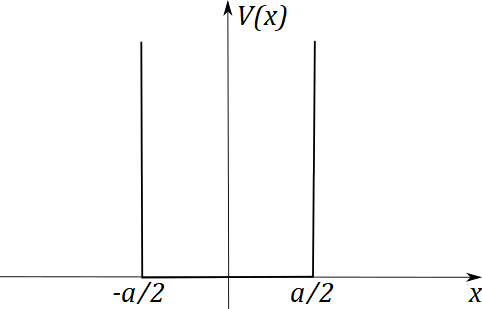
\includegraphics[width=\textwidth]{immagini/cap_9/fig_9_1.png}	
\end{minipage}
\begin{minipage}{.55\textwidth}
\begin{align}
V(x)= 
\begin{cases}
\infty \quad x<0,\\
0 \quad -a/2>x>a/2, \\
\infty \quad \textrm{fuori}.
\end{cases}
\\
\textrm{(buca di potenziale infinita)} \nonumber
\end{align}
\end{minipage}\\
In questo caso, infatti, il potenziale è una funzione pari delle coordinate e l'operatore hamiltoniano commuta con l'operatore di parità (1-dimensionale)
\begin{equation}
  \comm {H}{P}= 0
\end{equation}
Le autofunzioni di questa hamiltoniana si possono ottenere dalle autofunzioni calcolate nel caso della buca di potenziale infinita tra $x=0$ ed $x=a$ semplicemente traslando di $-a/2$ il valore della coordinata. Pertanto si trova
\begin{align}
  \psi_n(x) = \sqrt{\frac{2}{a}}\sin(\frac{n\pi}{a})\qty(x-\frac{a}{2})= \sqrt{\frac{2}{a}}\Im(e^{\frac{in\pi x}{a}}e^{-\frac{in\pi}{2}})=\nonumber\\
  =\sqrt{\frac{2}{a}}\qty[\sin(\frac{n\pi x}{a})\cos(\frac{n\pi}{2})-\cos(\frac{n\pi x}{a})\sin(\frac{n\pi}{2})] .
\end{align}
Si presentano allora due casi, a seconda che \emph{n} sia pari o dispari:
\begin{equation}
  \begin{cases}
    \psi_n(x)= (-1)^{n/2}\sqrt{\frac{2}{a}}\sin(\frac{n\pi x}{a}),\quad n=2,4,6,\;\dots\\
    \psi_n(x)= (-1)^{\frac{n+1}{2}}\sqrt{\frac{2}{a}}\cos(\frac{n\pi x}{a}),\quad n=1,3,5,\;\dots
  \end{cases}
\end{equation}
Senza perdere di generalità possiamo omettere in queste espressioni i fattori di fase irrilevanti e scrivere dunque:
\begin{equation}
  \begin{cases}
    \psi_n(x)= \sqrt{\frac{2}{a}}\sin(\frac{n\pi x}{a}),\quad n=2,4,6,\;\dots\\
    \psi_n(x)= \sqrt{\frac{2}{a}}\cos(\frac{n\pi x}{a}),\quad n=1,3,5,\;\dots
  \end{cases}
\end{equation}
Vediamo dunque che \textbf{le autofunzioni dell'hamiltoniana} sono funzioni pari o dispari delle coordinate, ossia \textbf{risultano simultaneamente autofunzioni dell'operatore di parità}.
